\documentclass[11pt,a4paper]{article}
\usepackage[margin=2.2cm]{geometry}
\usepackage{fontspec}
\setmainfont{Arial}
\setsansfont{Arial}
\usepackage[spanish,es-nodecimaldot]{babel}
\usepackage{amsmath}
\usepackage{graphicx}
\usepackage{booktabs,tabularx,array}
\usepackage{float}
\usepackage{xcolor}
\usepackage{hyperref}
\usepackage{fancyhdr}
\usepackage{enumitem}
\usepackage{caption}
\usepackage{microtype}

\definecolor{azul}{HTML}{174A6E}
\hypersetup{colorlinks=true,linkcolor=azul,urlcolor=azul,pdftitle={Modelos, métricas y gráficos del sistema DMI TerraBovina}}
\pagestyle{fancy}
\fancyhf{}
\lhead{Modelo DMI TerraBovina}
\rhead{Modelos, métricas y gráficos}
\cfoot{\thepage}
\setlength{\headheight}{14pt}
\setlength{\parindent}{0pt}
\setlength{\parskip}{5pt}
\setlist{nosep,leftmargin=1.4em}
\captionsetup{font=small,labelfont=bf}
\newcommand{\codigo}[1]{\texttt{\detokenize{#1}}}

\begin{document}

{\LARGE\bfseries Modelo DMI TerraBovina: funcionamiento, comparación de modelos, métricas y gráficos}\par
\vspace{0.4em}
{\large Documento técnico resumido}\par
\vspace{0.7em}
Este documento explica de forma precisa qué hace el sistema, por qué se evaluó cada algoritmo, cómo se interpretan sus métricas y qué información aporta cada gráfico. Los valores corresponden al código y a \codigo{reports/model_metrics.json} del repositorio analizado.

\tableofcontents

\section{¿Qué hace el modelo?}

El sistema estima el \textbf{consumo diario de materia seca} de un bovino. La salida principal es \codigo{dmi_kg_dia}, expresada en kilogramos de materia seca por animal y día. Se trata de un problema de \textbf{regresión supervisada}: durante el entrenamiento, el algoritmo observa animales cuyas características y consumo real son conocidos; a partir de esos ejemplos aprende una relación matemática para predecir el consumo de nuevos animales.

Las cuatro entradas son:
\begin{itemize}
  \item \codigo{peso_vivo_kg}: peso vivo del animal;
  \item \codigo{categoria_terrabovina}: Vaca, Vaquilla, Novillo, Toro o Ternero/Ternera;
  \item \codigo{condicion_corporal}: indicador numérico de condición corporal;
  \item \codigo{estado_fisiologico_norm}: estado fisiológico normalizado.
\end{itemize}

La condición corporal y el estado fisiológico se conservan únicamente para vacas. En las demás categorías, la condición pasa a ausente y el estado a DESCONOCIDO, porque esas variables tienen demasiados faltantes fuera del grupo Vaca.

Antes de entrenar, los valores numéricos ausentes se imputan con la mediana y se estandarizan. Las variables categóricas se convierten mediante \textit{one-hot encoding}. No se utilizan identificadores, fechas, periodo ni \codigo{dmi_pct_peso_vivo}. Esta última variable se calcula con el consumo real y usarla como entrada revelaría indirectamente el objetivo, produciendo fuga de información.

El dataset contiene 3.833 observaciones de 131 hogares o fincas de Bomet, Kenia. Para evaluar el sistema se aplican cinco folds de \codigo{StratifiedGroupKFold}. Todas las observaciones de un hogar permanecen en un único lado de cada división. Así, el modelo es evaluado con hogares que no utilizó para entrenar dentro de ese fold.

Una vez elegido el ganador, se entrena nuevamente con las 3.833 observaciones y se guarda en \codigo{models/dmi_model.joblib}. En inferencia devuelve, por animal, el DMI en kg/día y como porcentaje del peso vivo. También advierte cuando el peso se encuentra fuera del rango histórico de su categoría.

\section{¿Por qué se compararon estos modelos?}

La comparación incluye cuatro candidatos con niveles crecientes de complejidad. No se eligieron porque todos fueran necesarios para producción, sino porque permiten responder preguntas diferentes sobre los datos.

\subsection{Baseline de la media}

\textbf{Configuración:} \codigo{DummyRegressor(strategy="mean")}.

Predice la media del consumo observado en el conjunto de entrenamiento. No aprende relaciones con peso, categoría o estado fisiológico. Su función es actuar como \textbf{referencia mínima}: permite comprobar si los modelos verdaderos aportan información por encima de una predicción ingenua.

\textbf{Por qué fue elegido para la comparación:} sin baseline, un error aparentemente bajo carece de contexto. Si Ridge, Random Forest o CatBoost no superaran claramente a la media, el proyecto no demostraría capacidad predictiva útil.

\textbf{Ventaja:} extremadamente simple, rápido y fácil de interpretar. \textbf{Desventaja:} entrega prácticamente la misma estimación a todos los animales y no personaliza el consumo.

\subsection{Regresión Ridge}

\textbf{Configuración:} pipeline de preprocesamiento más \codigo{Ridge(alpha=10.0)}.

Ridge es una regresión lineal con penalización L2. Ajusta una suma de efectos de las variables y penaliza coeficientes excesivamente grandes:
\begin{equation}
\min_{\beta_0,\boldsymbol{\beta}}\sum_{i=1}^{n}(y_i-\beta_0-\mathbf{x}_i^T\boldsymbol{\beta})^2+\alpha\sum_{j=1}^{p}\beta_j^2.
\end{equation}

El valor $\alpha=10$ controla la intensidad de regularización. Esto reduce sensibilidad al ruido y a la colinealidad producida por variables categóricas codificadas. Ridge supone una relación principalmente lineal y aditiva, pero puede representar diferencias entre categorías y estados mediante sus coeficientes.

\textbf{Por qué fue elegido para la comparación:} el peso vivo tiene una asociación lineal fuerte con el DMI. Ridge permite comprobar si una relación relativamente simple es suficiente, ofrece predicciones suaves y es más interpretable que los árboles.

\textbf{Ventajas:} rapidez, estabilidad, tamaño reducido e inspección directa de coeficientes. \textbf{Desventajas:} captura con dificultad umbrales, interacciones y curvas complejas si no se agregan características específicas.

\subsection{Random Forest}

\textbf{Configuración:} 100 árboles, profundidad máxima 10 y semilla 42.

Random Forest combina muchos árboles de decisión. Cada árbol divide el espacio de características mediante reglas; el bosque promedia sus resultados. Puede detectar relaciones no lineales e interacciones sin escribirlas manualmente.

\textbf{Por qué fue elegido para la comparación:} permite comprobar si existen patrones por rangos de peso, categorías o interacciones que un modelo lineal no logra representar. Funciona como alternativa no lineal clásica y robusta.

\textbf{Ventajas:} flexibilidad, captura de interacciones y poca dependencia de supuestos lineales. \textbf{Desventajas:} menor interpretabilidad, mayor tamaño y predicciones por regiones. Los árboles no extrapolan bien una tendencia continua más allá de los rangos observados.

\subsection{CatBoost}

\textbf{Configuración:} 500 iteraciones, profundidad 6, tasa de aprendizaje 0,04, pérdida RMSE y semilla 42.

CatBoost construye árboles secuencialmente. Cada nuevo árbol intenta corregir parte del error acumulado por los anteriores. Está especialmente diseñado para trabajar con variables categóricas y reducir problemas de codificación y sobreajuste asociados a ellas.

\textbf{Por qué fue elegido para la comparación:} es la alternativa no lineal más sofisticada del proyecto y permite evaluar si el boosting y el tratamiento directo de categorías mejoran el rendimiento frente a Ridge y Random Forest.

\textbf{Ventajas:} gran capacidad para relaciones complejas, interacciones y categorías. \textbf{Desventajas:} mayor costo computacional, más hiperparámetros, menor transparencia y riesgo de aprender ruido si no se valida correctamente.

\section{Comparación de resultados}

\begin{table}[H]
\centering
\caption{Resultados globales obtenidos con predicciones fuera de fold.}
\begin{tabular}{lrrr}
\toprule
\textbf{Modelo} & \textbf{MAE} & \textbf{RMSE} & \textbf{$R^2$}\\
\midrule
Baseline media & 2,1280 & 2,7273 & -0,0029\\
\textbf{Ridge} & \textbf{1,1019} & \textbf{1,5354} & \textbf{0,6821}\\
Random Forest & 1,1611 & 1,6458 & 0,6348\\
CatBoost & 1,1027 & 1,5587 & 0,6724\\
\bottomrule
\end{tabular}
\end{table}

\textbf{Baseline:} su MAE de 2,1280 muestra el error de predecir aproximadamente un promedio. Su $R^2$ negativo confirma que no explica adecuadamente las diferencias individuales.

\textbf{Ridge:} consigue el menor MAE y RMSE y el mayor $R^2$. Reduce el MAE del baseline alrededor de 48,2\%. Es el ganador formal porque el código selecciona exclusivamente el menor MAE.

\textbf{Random Forest:} mejora ampliamente al baseline, pero queda por detrás de Ridge: su MAE es 0,0592 kg/día mayor y su $R^2$ es 0,0473 menor. La flexibilidad adicional no produjo una mejora global; posiblemente la señal principal pueda describirse razonablemente con una estructura lineal regularizada.

\textbf{CatBoost:} queda prácticamente empatado con Ridge. Su MAE es solo 0,0008 kg/día mayor. También tiene RMSE 0,0233 superior y $R^2$ 0,0097 inferior. La diferencia de MAE es demasiado pequeña para afirmar superioridad estadística sin intervalos de confianza o pruebas pareadas.

\subsection{¿Por qué se eligió Ridge?}

Ridge se seleccionó porque la regla implementada elige automáticamente el modelo con menor MAE. Además, también obtiene el menor RMSE y el mayor $R^2$. Entre dos desempeños casi idénticos, Ridge agrega ventajas prácticas: es más simple, rápido, pequeño e interpretable que CatBoost. Por eso su elección es razonable.

La formulación correcta no es ``Ridge es claramente superior a todos'', sino: \textbf{Ridge fue el ganador numérico y práctico, mientras que CatBoost alcanzó un rendimiento esencialmente equivalente}. No se realizó una prueba estadística que demuestre que los 0,0008 kg/día de diferencia se mantendrían con otra muestra.

\subsection{Comparación por categoría}

\begin{table}[H]
\centering
\caption{MAE de los tres modelos predictivos por categoría.}
\begin{tabular}{lrrr}
\toprule
\textbf{Categoría} & \textbf{Ridge} & \textbf{Random Forest} & \textbf{CatBoost}\\
\midrule
Vaca & \textbf{1,5857} & 1,6903 & 1,5992\\
Vaquilla & \textbf{0,7540} & 0,8339 & 0,7732\\
Novillo & 0,6639 & \textbf{0,6563} & 0,6608\\
Toro & \textbf{1,0204} & 1,0924 & 1,0647\\
Ternero/Ternera & 0,5846 & 0,5469 & \textbf{0,5294}\\
\bottomrule
\end{tabular}
\end{table}

Ridge domina Vaca, Vaquilla y Toro. Random Forest obtiene una ventaja pequeña en Novillo y CatBoost es mejor en Ternero/Ternera. Esto demuestra que seleccionar por promedio global no significa ganar en cada subgrupo. El mayor MAE de Ridge aparece en vacas, que también tienen el mayor consumo y la mayor dispersión.

\section{Cómo se interpretan las métricas}

\subsection{MAE: error absoluto medio}

\begin{equation}
MAE=\frac{1}{n}\sum_{i=1}^{n}|y_i-\hat y_i|.
\end{equation}

\textbf{Cómo se lee:} indica cuántos kilogramos de materia seca por día se desvía, en promedio, una predicción respecto del valor real, ignorando el signo del error. Menor es mejor; cero sería perfecto.

El MAE de Ridge, 1,1019 kg MS/día, significa que el error absoluto promedio de sus predicciones fuera de fold es aproximadamente 1,10 kg diarios. No significa que todas fallen exactamente 1,10 kg: algunas se acercan más y otras se alejan considerablemente.

\textbf{¿Es bueno?} Es claramente mejor que el baseline de 2,1280 y reduce su error casi a la mitad. En relación con el DMI medio global de 4,8285 kg/día, 1,1019 representa aproximadamente 22,8\%, aunque esa razón no es una métrica oficial y cambia según categoría. Es un resultado útil como prueba técnica, pero todavía considerable para decisiones nutricionales precisas, especialmente en vacas, cuyo MAE es 1,5857.

\subsection{RMSE: raíz del error cuadrático medio}

\begin{equation}
RMSE=\sqrt{\frac{1}{n}\sum_{i=1}^{n}(y_i-\hat y_i)^2}.
\end{equation}

\textbf{Cómo se lee:} también se expresa en kg MS/día, pero elevar al cuadrado hace que los errores grandes pesen más. Menor es mejor y cero sería perfecto.

Ridge obtiene RMSE 1,5354. Es mayor que su MAE de 1,1019, lo que indica que existen predicciones con errores grandes que aumentan el promedio cuadrático. El RMSE permite distinguir modelos con MAE parecido: Ridge y CatBoost casi empatan en MAE, pero Ridge presenta un RMSE menor, señal favorable respecto de errores elevados.

\textbf{¿Es bueno?} Es 43,7\% menor que el RMSE del baseline. El resultado es sólido internamente, pero la distancia entre RMSE y MAE muestra que todavía hay casos difíciles y que no conviene comunicar únicamente el error promedio.

\subsection{$R^2$: coeficiente de determinación}

\begin{equation}
R^2=1-\frac{\sum_i(y_i-\hat y_i)^2}{\sum_i(y_i-\bar y)^2}.
\end{equation}

\textbf{Cómo se lee:} mide cuánto mejora el modelo respecto de usar la media para representar la variabilidad. Un valor cercano a 1 es mejor; 0 se parece a predecir la media; un valor negativo indica un resultado peor que esa referencia bajo la evaluación considerada.

El $R^2$ de Ridge es 0,6821. Puede expresarse de manera aproximada como que el modelo representa el 68,21\% de la variabilidad del DMI presente en estas predicciones fuera de fold. No significa que acierte el 68,21\% de los animales ni que tenga una precisión de 68,21\%.

\textbf{¿Es bueno?} Un 0,6821 representa capacidad explicativa moderada-alta para este dataset y es muy superior al baseline de -0,0029. Aun así, aproximadamente 31,8\% de la variabilidad queda sin representar por el modelo, posiblemente por ruido, variables omitidas y relaciones no capturadas. En vacas, el $R^2$ baja a 0,4110, por lo que la calidad no es uniforme.

\subsection{Lectura conjunta}

Ninguna métrica debe interpretarse sola. MAE da el error cotidiano más intuitivo; RMSE advierte sobre errores grandes; $R^2$ indica capacidad relativa para representar variabilidad. Ridge es consistente en las tres: menor error típico, menor penalización por errores grandes y mayor capacidad explicativa. Sin embargo, las métricas provienen del mismo dataset de Kenia y no garantizan el mismo rendimiento en otro país o sistema productivo.

\section{Explicación de los gráficos}

\subsection{Comparación de modelos}

\begin{figure}[H]
\centering
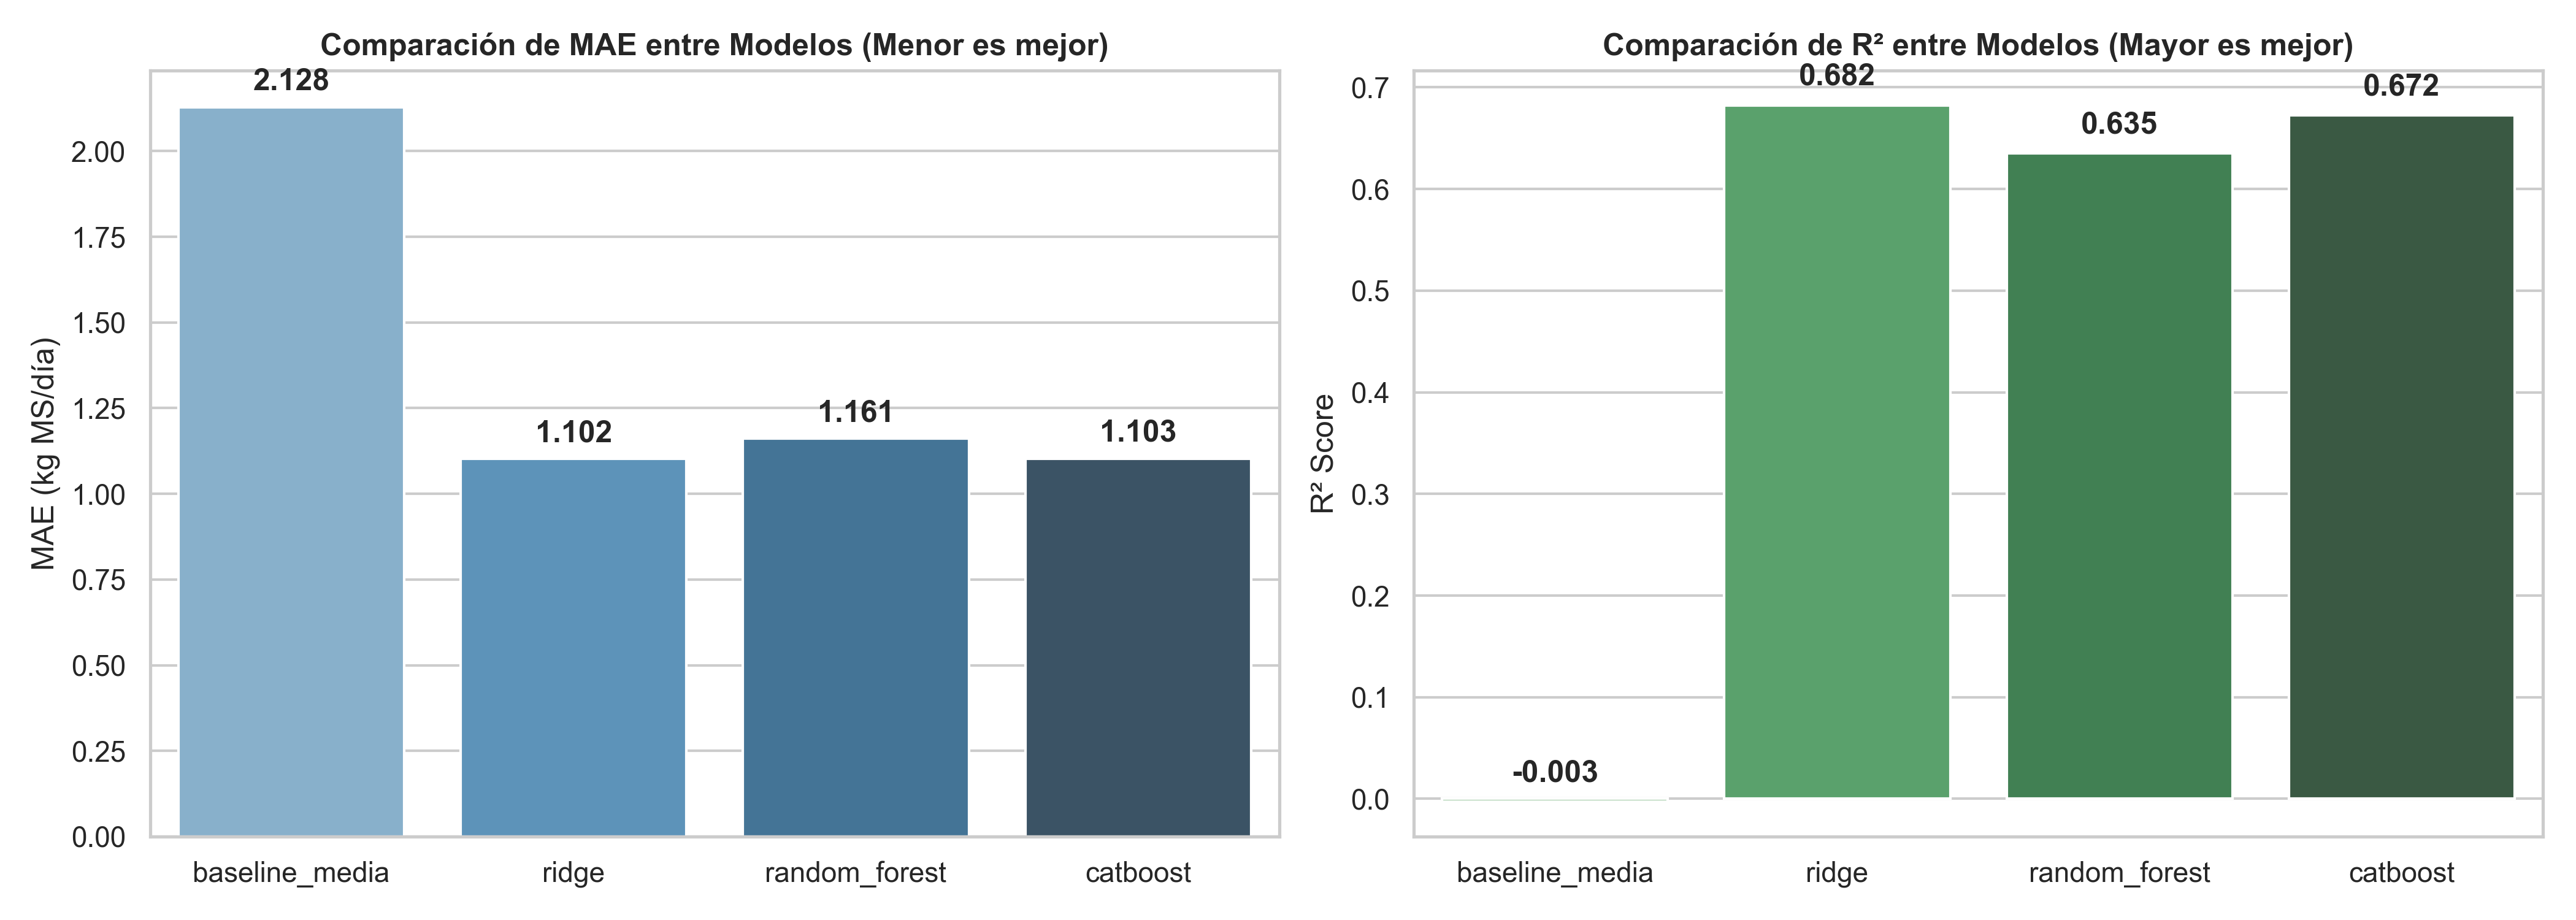
\includegraphics[width=\textwidth]{figures/1_model_comparison_mae_r2.png}
\caption{Comparación de MAE y $R^2$ entre candidatos.}
\end{figure}

El panel izquierdo muestra MAE: una barra más baja es mejor. El baseline es claramente peor; Ridge y CatBoost casi coinciden; Random Forest queda en una posición intermedia. El panel derecho muestra $R^2$: una barra más alta es mejor. Ridge encabeza la comparación, seguido muy cerca por CatBoost. El gráfico justifica la selección formal, pero también hace visible el empate práctico.

\subsection{Valores reales frente a predichos}

\begin{figure}[H]
\centering
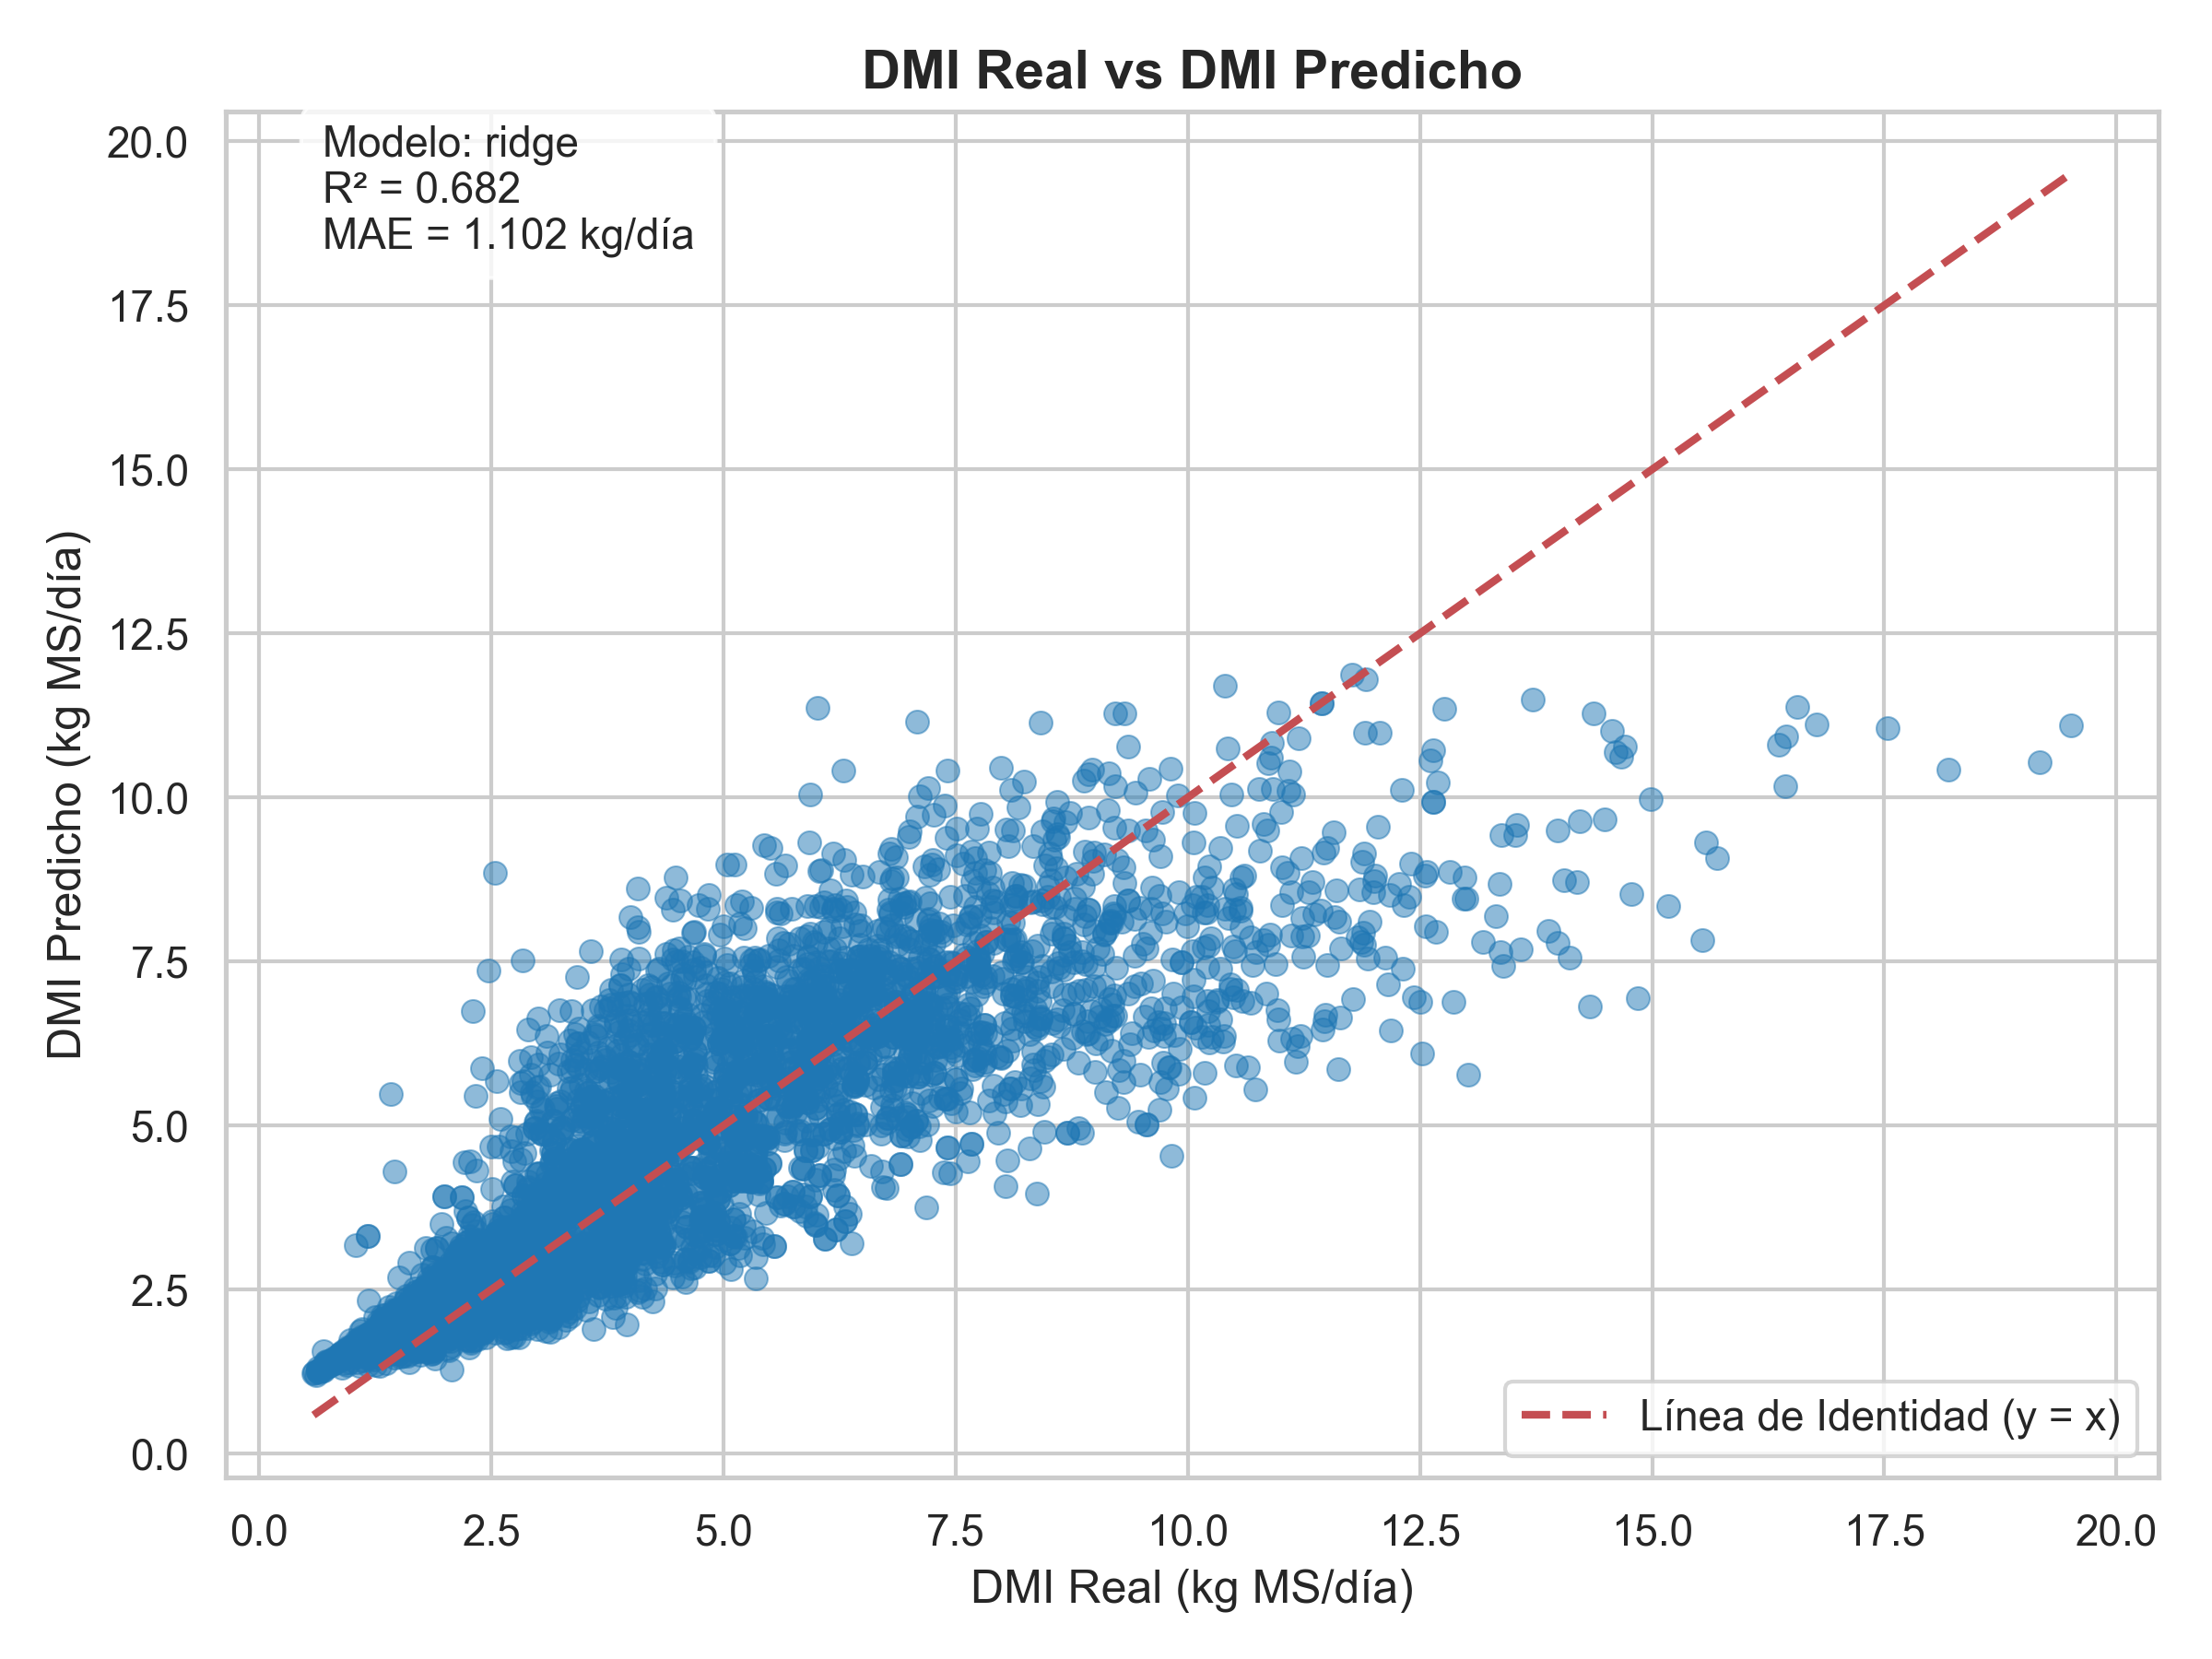
\includegraphics[width=0.78\textwidth]{figures/2_actual_vs_predicted.png}
\caption{DMI real en el eje horizontal y DMI predicho en el vertical.}
\end{figure}

Cada punto es una observación. La línea diagonal representa una predicción perfecta. Cuanto más cerca está un punto de la línea, menor es su error. La nube sigue una tendencia positiva, por lo que el modelo distingue consumos bajos y altos. Sin embargo, para DMI reales muy elevados, muchas predicciones quedan por debajo de la diagonal: Ridge tiende a acercar valores extremos hacia el promedio. Este patrón ayuda a explicar el mayor error en vacas de consumo alto.

\subsection{Distribución de residuos}

\begin{figure}[H]
\centering
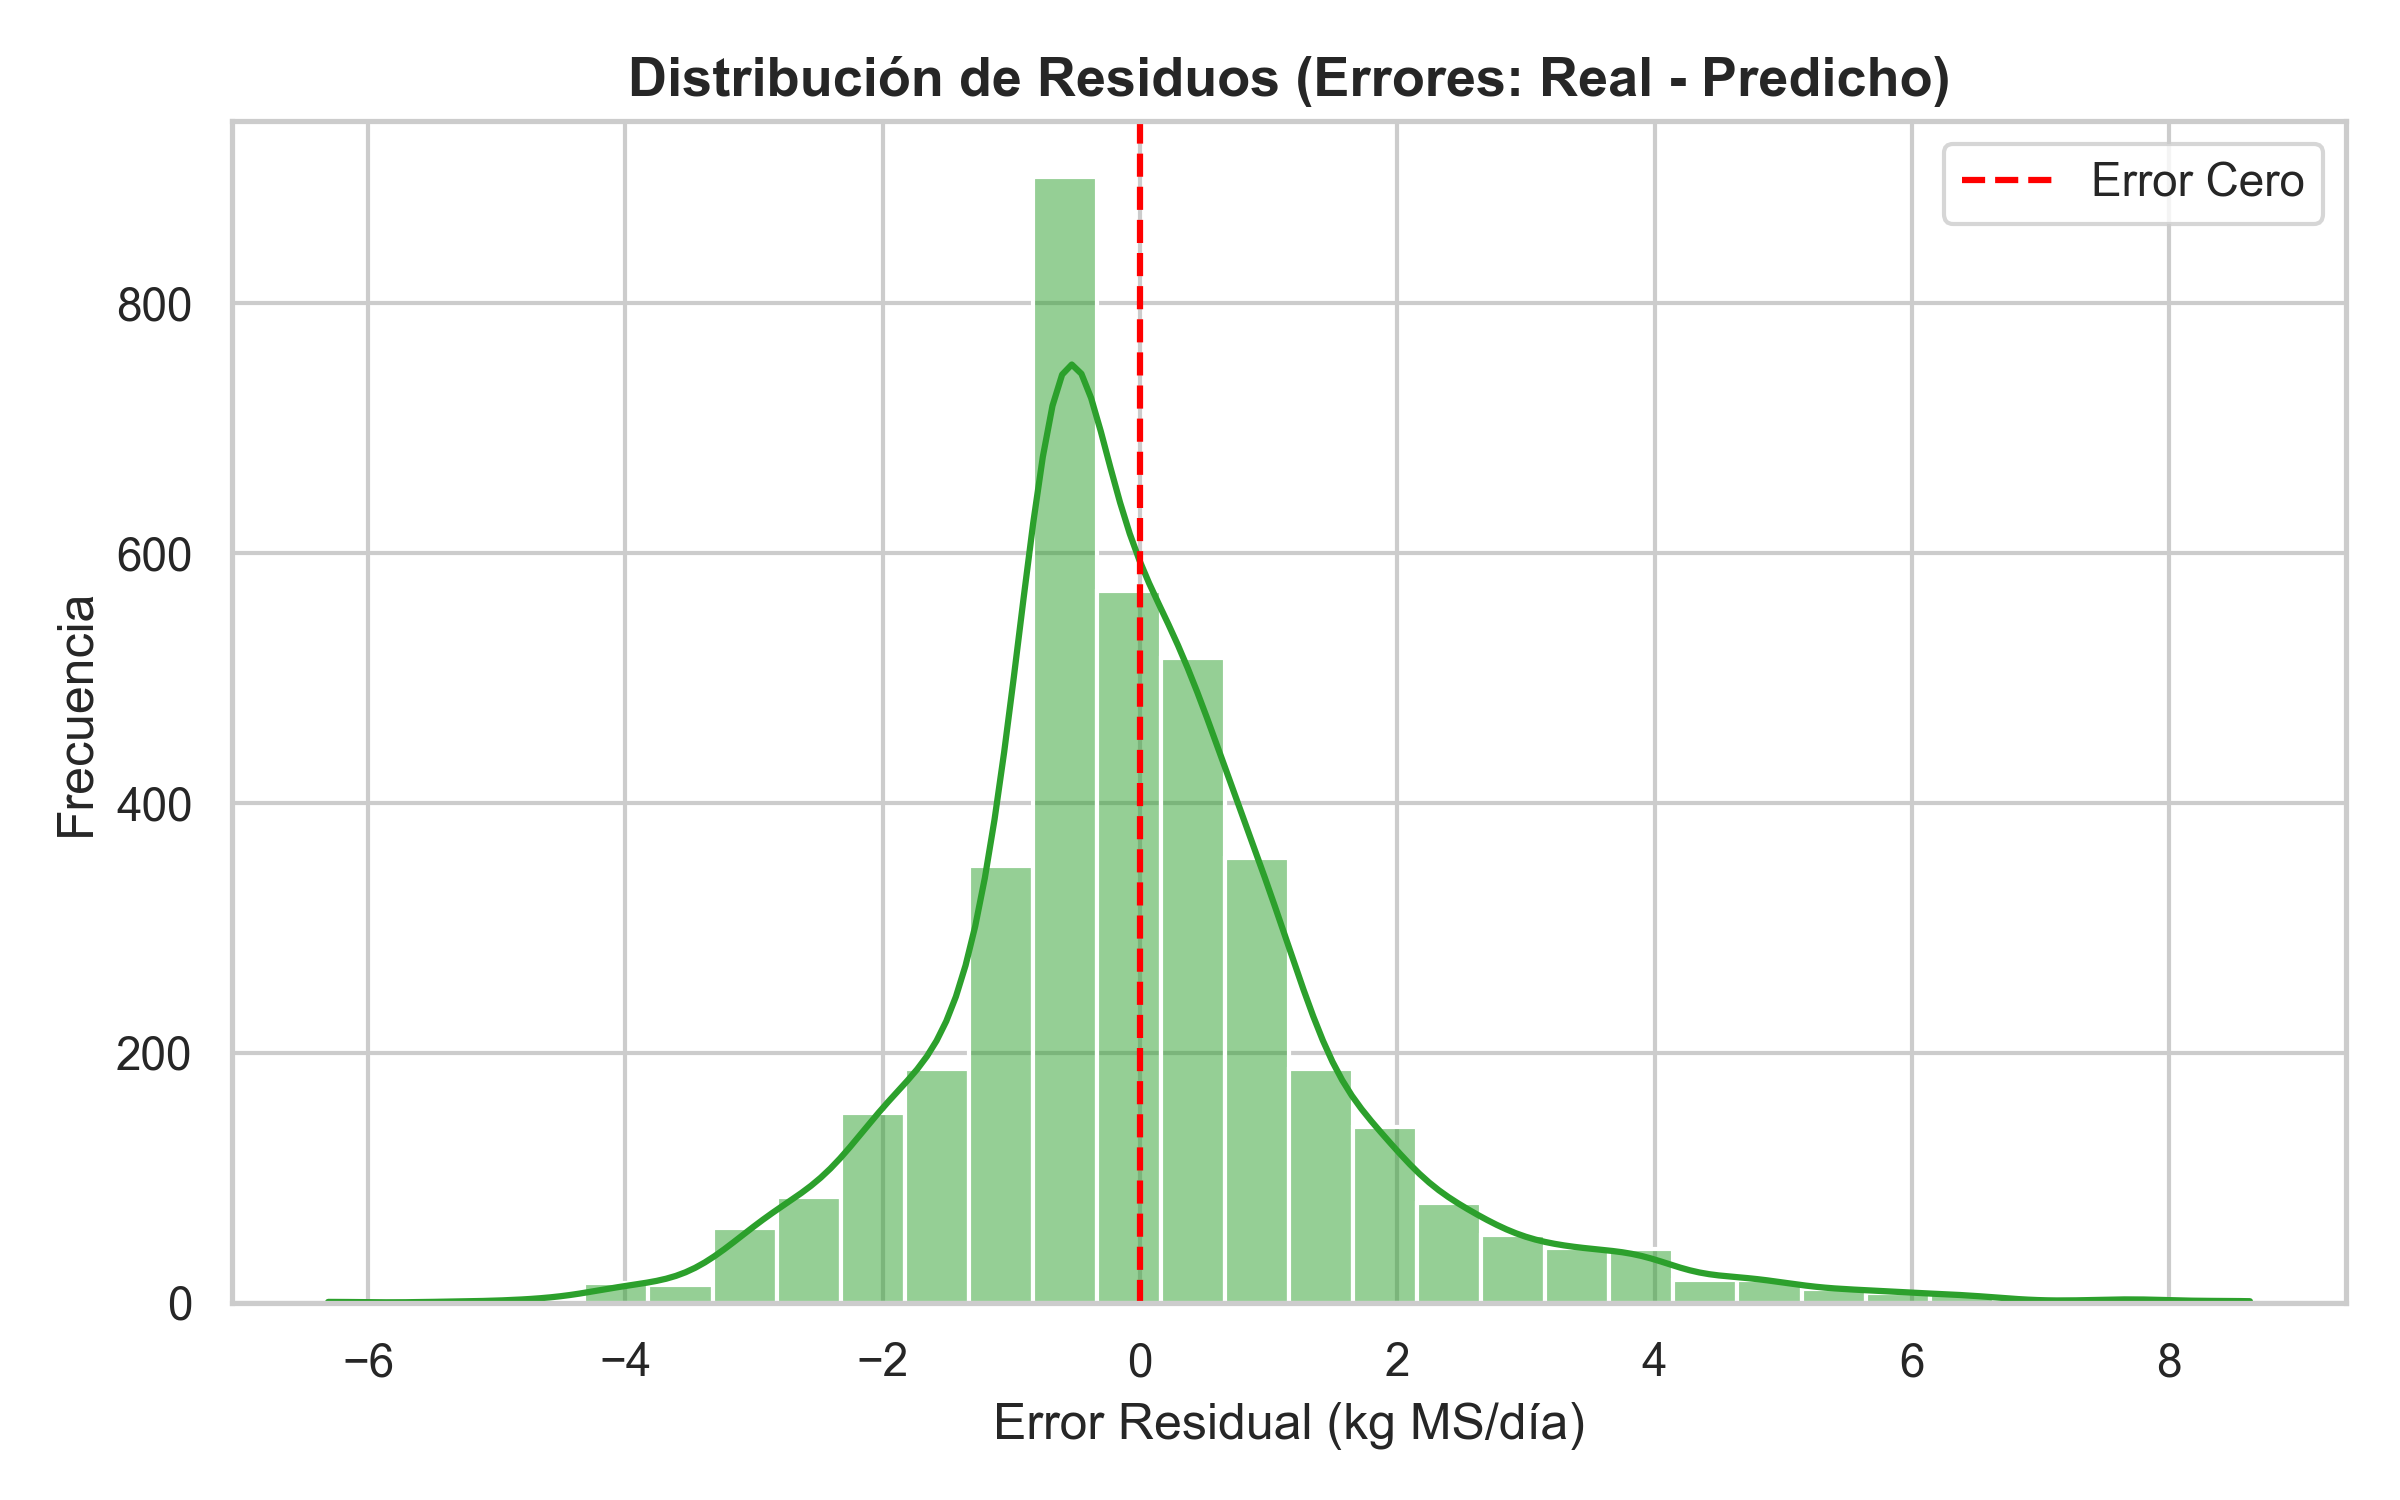
\includegraphics[width=0.82\textwidth]{figures/3_residuals_distribution.png}
\caption{Distribución del error definido como valor real menos valor predicho.}
\end{figure}

La línea roja en cero indica ausencia de error. Un residuo positivo significa que el modelo predijo menos que el consumo real; uno negativo significa sobreestimación. La mayor densidad está cerca de cero, señal favorable. La distribución posee colas y no es perfectamente simétrica; existen errores grandes en ambos sentidos, con una cola positiva visible. El histograma no demuestra por sí solo normalidad ni ausencia de sesgo por nivel de consumo.

\subsection{Coeficientes o importancia de variables}

\begin{figure}[H]
\centering
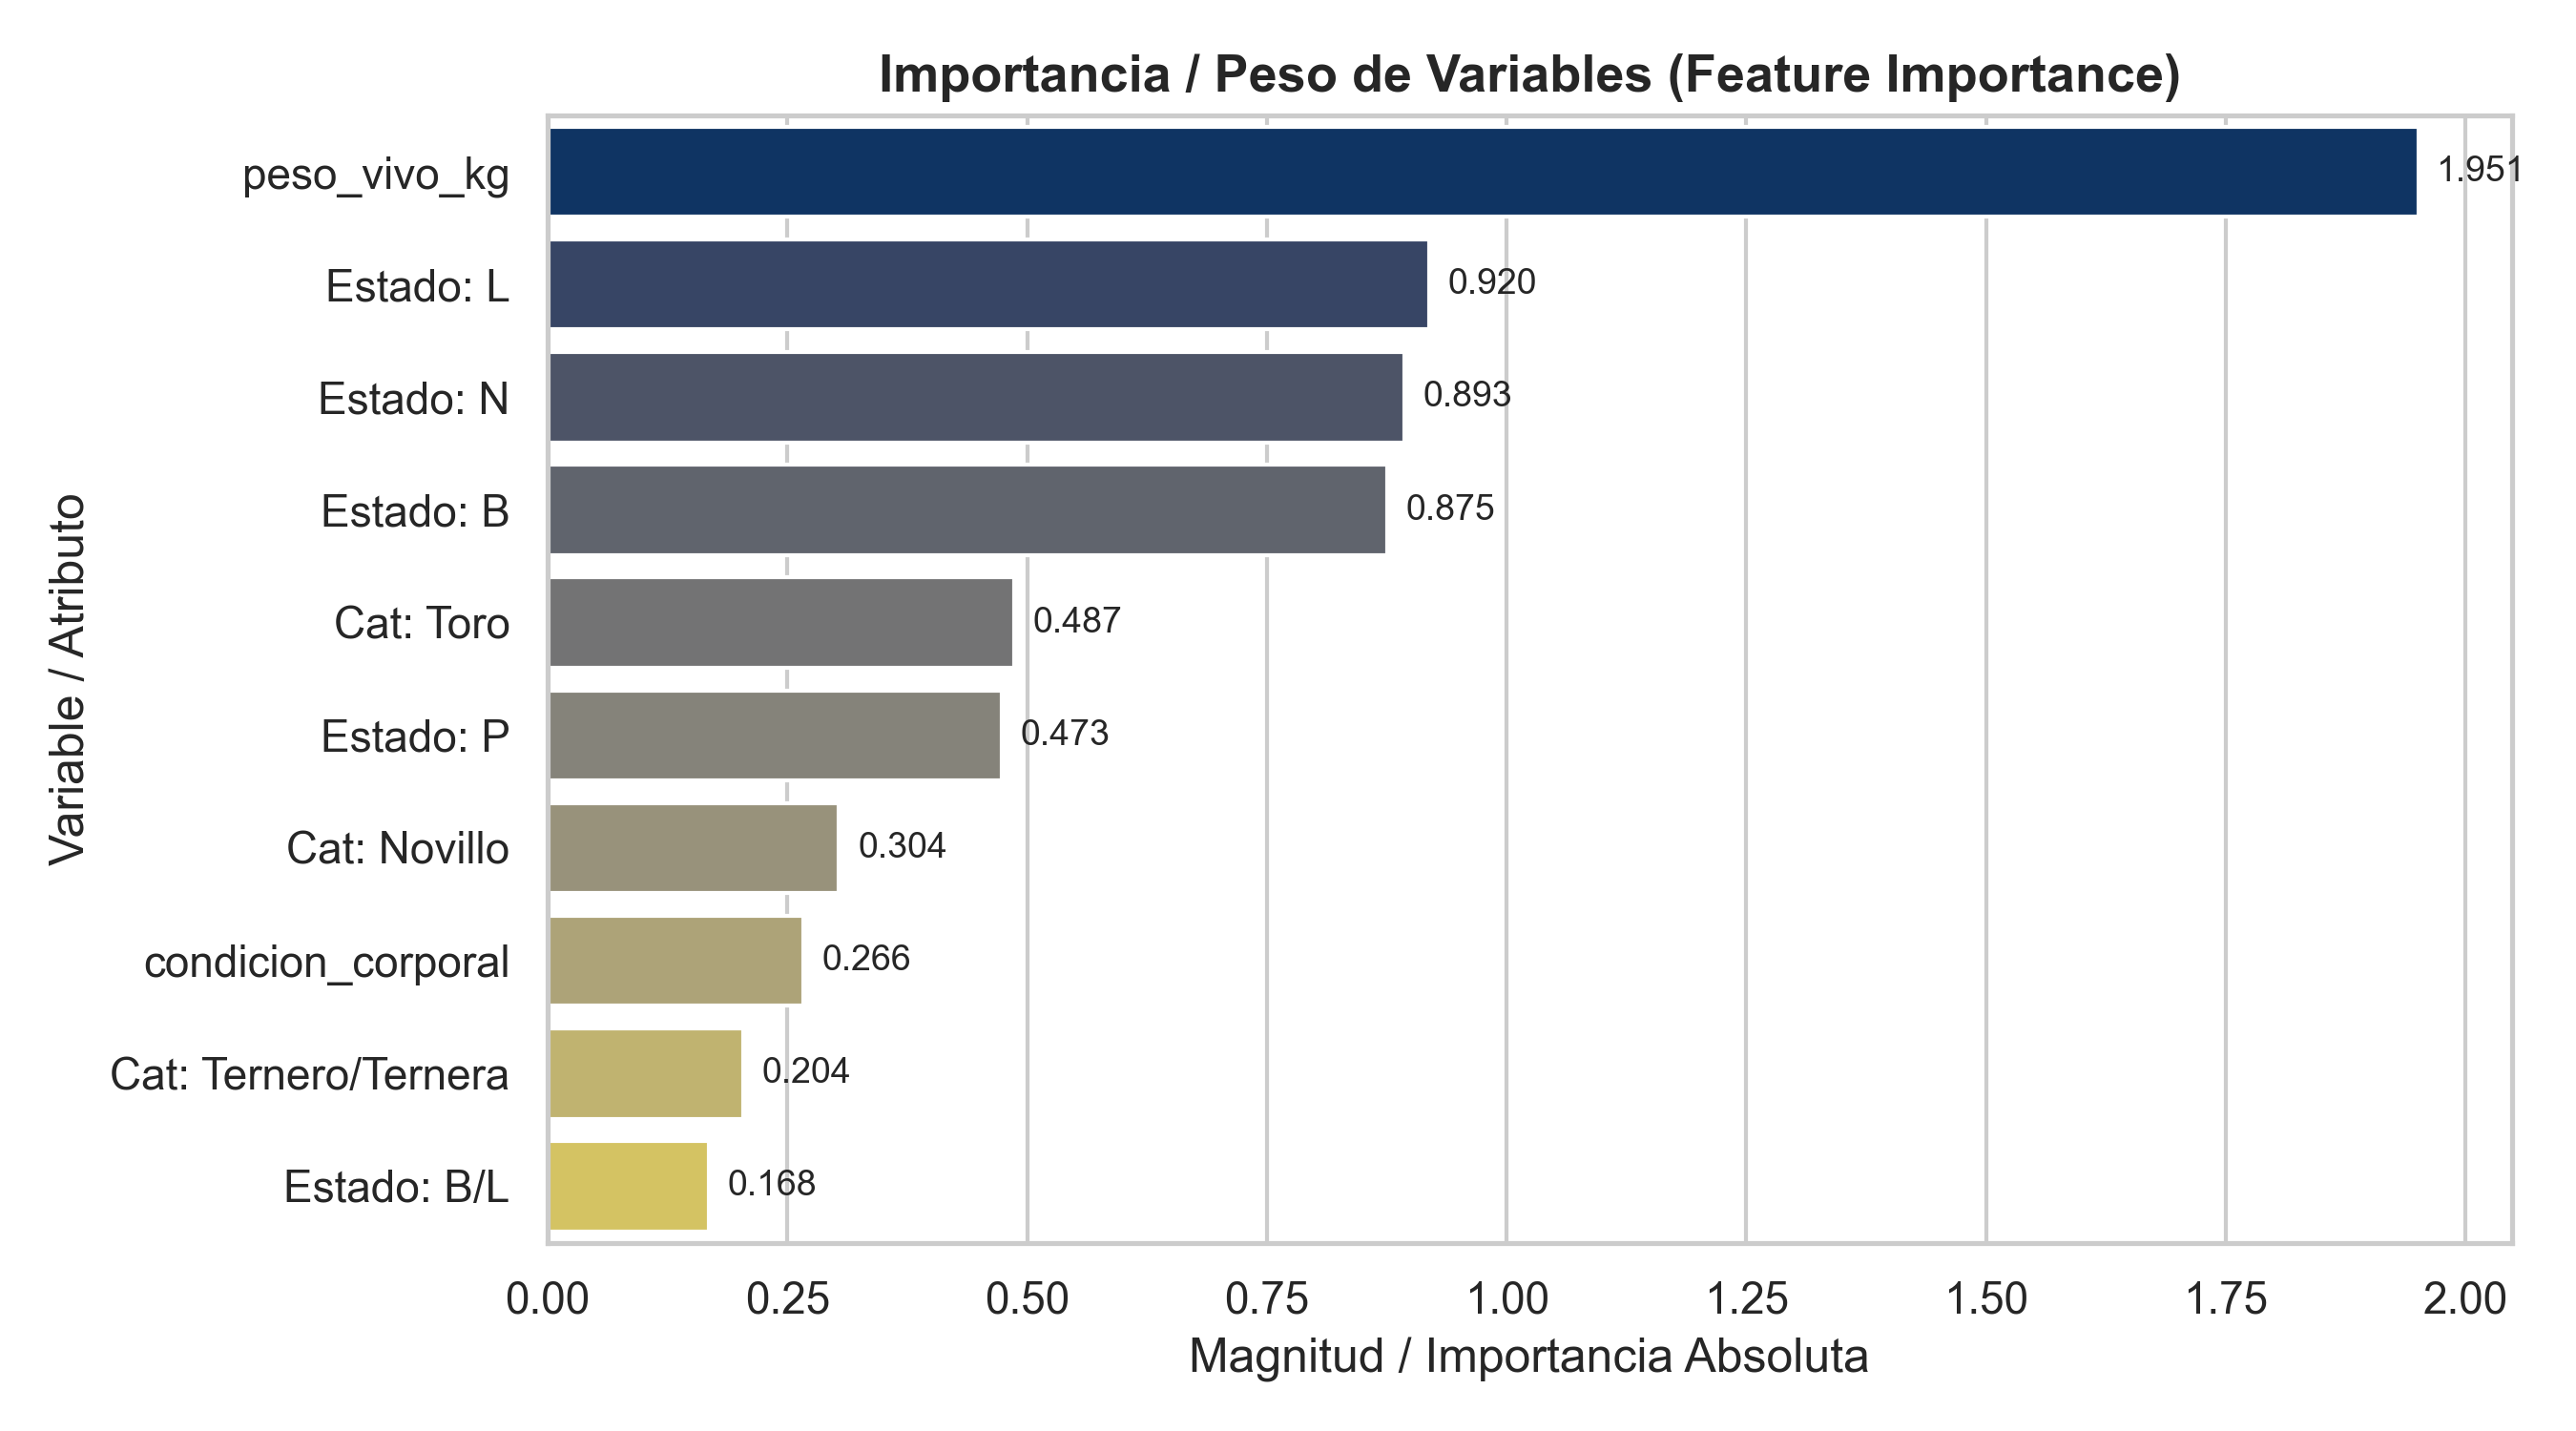
\includegraphics[width=0.85\textwidth]{figures/4_feature_importance.png}
\caption{Magnitud absoluta de los principales coeficientes de Ridge.}
\end{figure}

La barra más larga corresponde al peso vivo, confirmando que es la señal dominante. Después aparecen estados fisiológicos y categorías. El gráfico usa valores absolutos, por lo que no muestra si el efecto es positivo o negativo. Además, el peso fue estandarizado: su coeficiente representa una desviación estándar, no un kilogramo. Estas barras muestran peso matemático dentro del modelo, no importancia causal ni efecto biológico demostrado.

\subsection{MAE por categoría}

\begin{figure}[H]
\centering
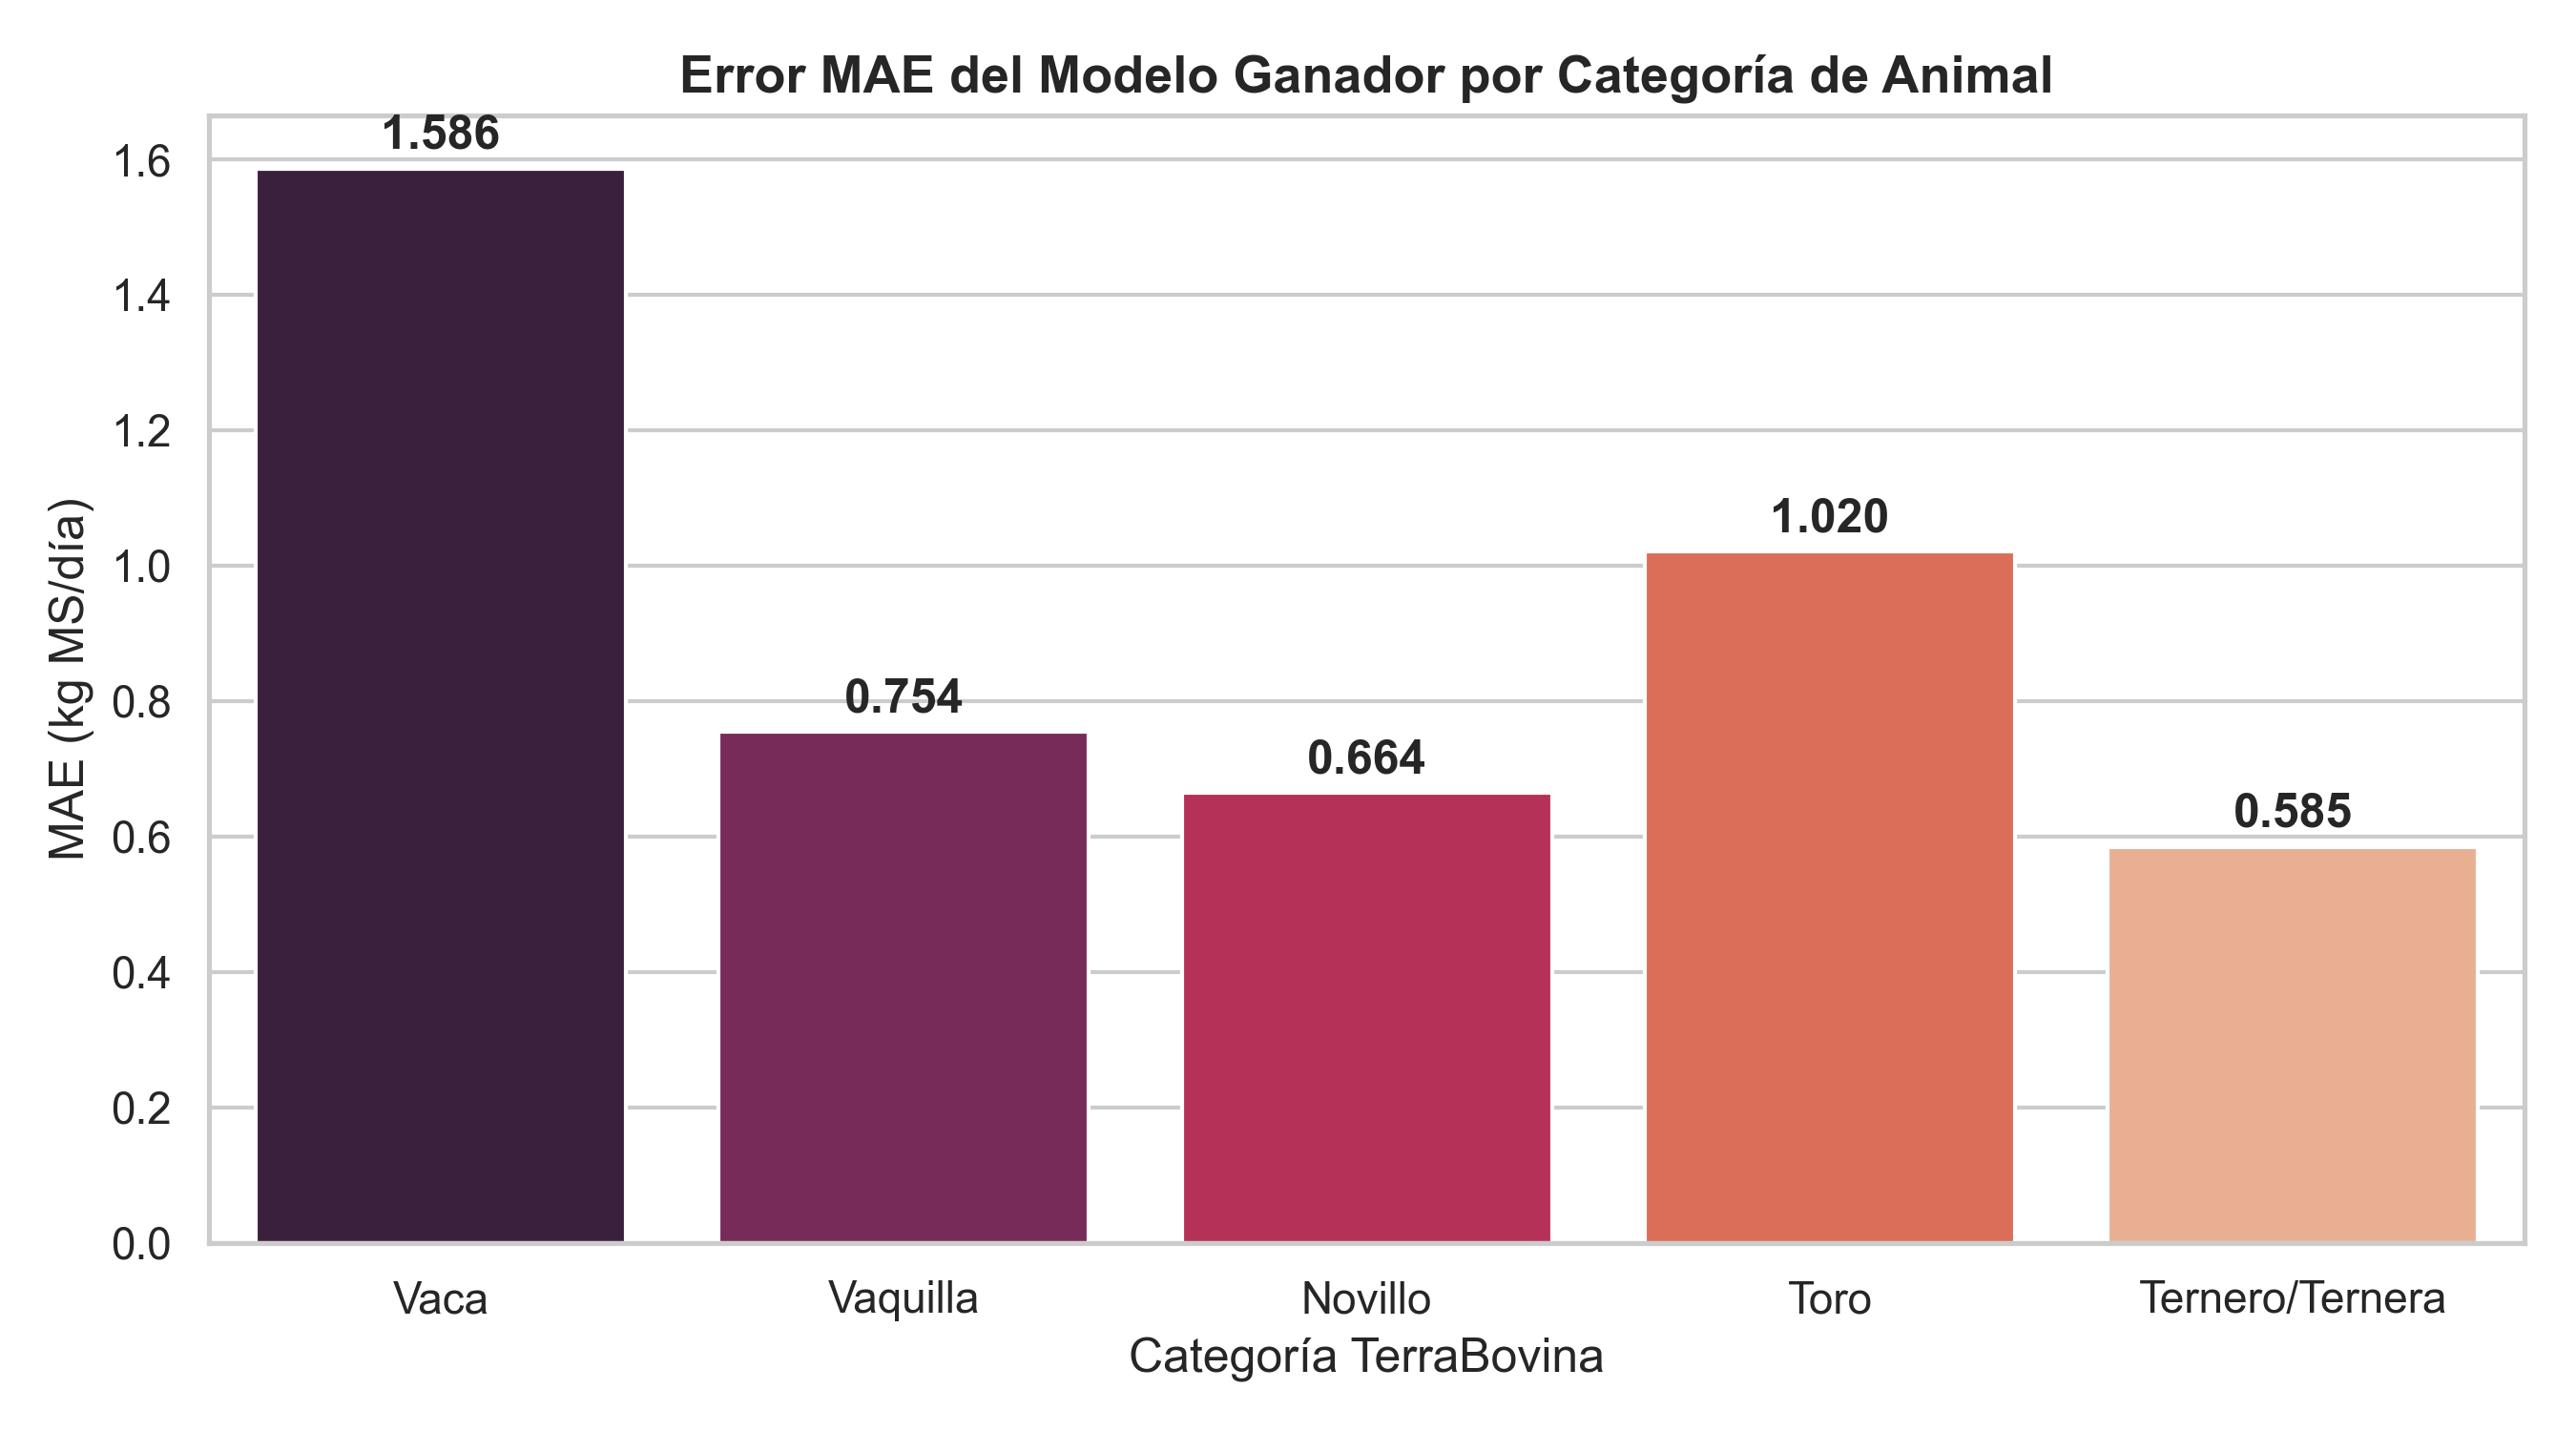
\includegraphics[width=0.88\textwidth]{figures/5_mae_by_category.png}
\caption{Error absoluto medio de Ridge por categoría animal.}
\end{figure}

Una barra más baja indica menor error absoluto. Ternero/Ternera presenta el menor MAE y Vaca el mayor. No debe concluirse directamente que el modelo ``entiende peor'' a las vacas sin considerar escala: las vacas tienen mayor DMI y dispersión. El gráfico sí demuestra que el error práctico en kg/día no es uniforme y que una única métrica global oculta diferencias importantes.

\subsection{Peso vivo frente a DMI}

\begin{figure}[H]
\centering
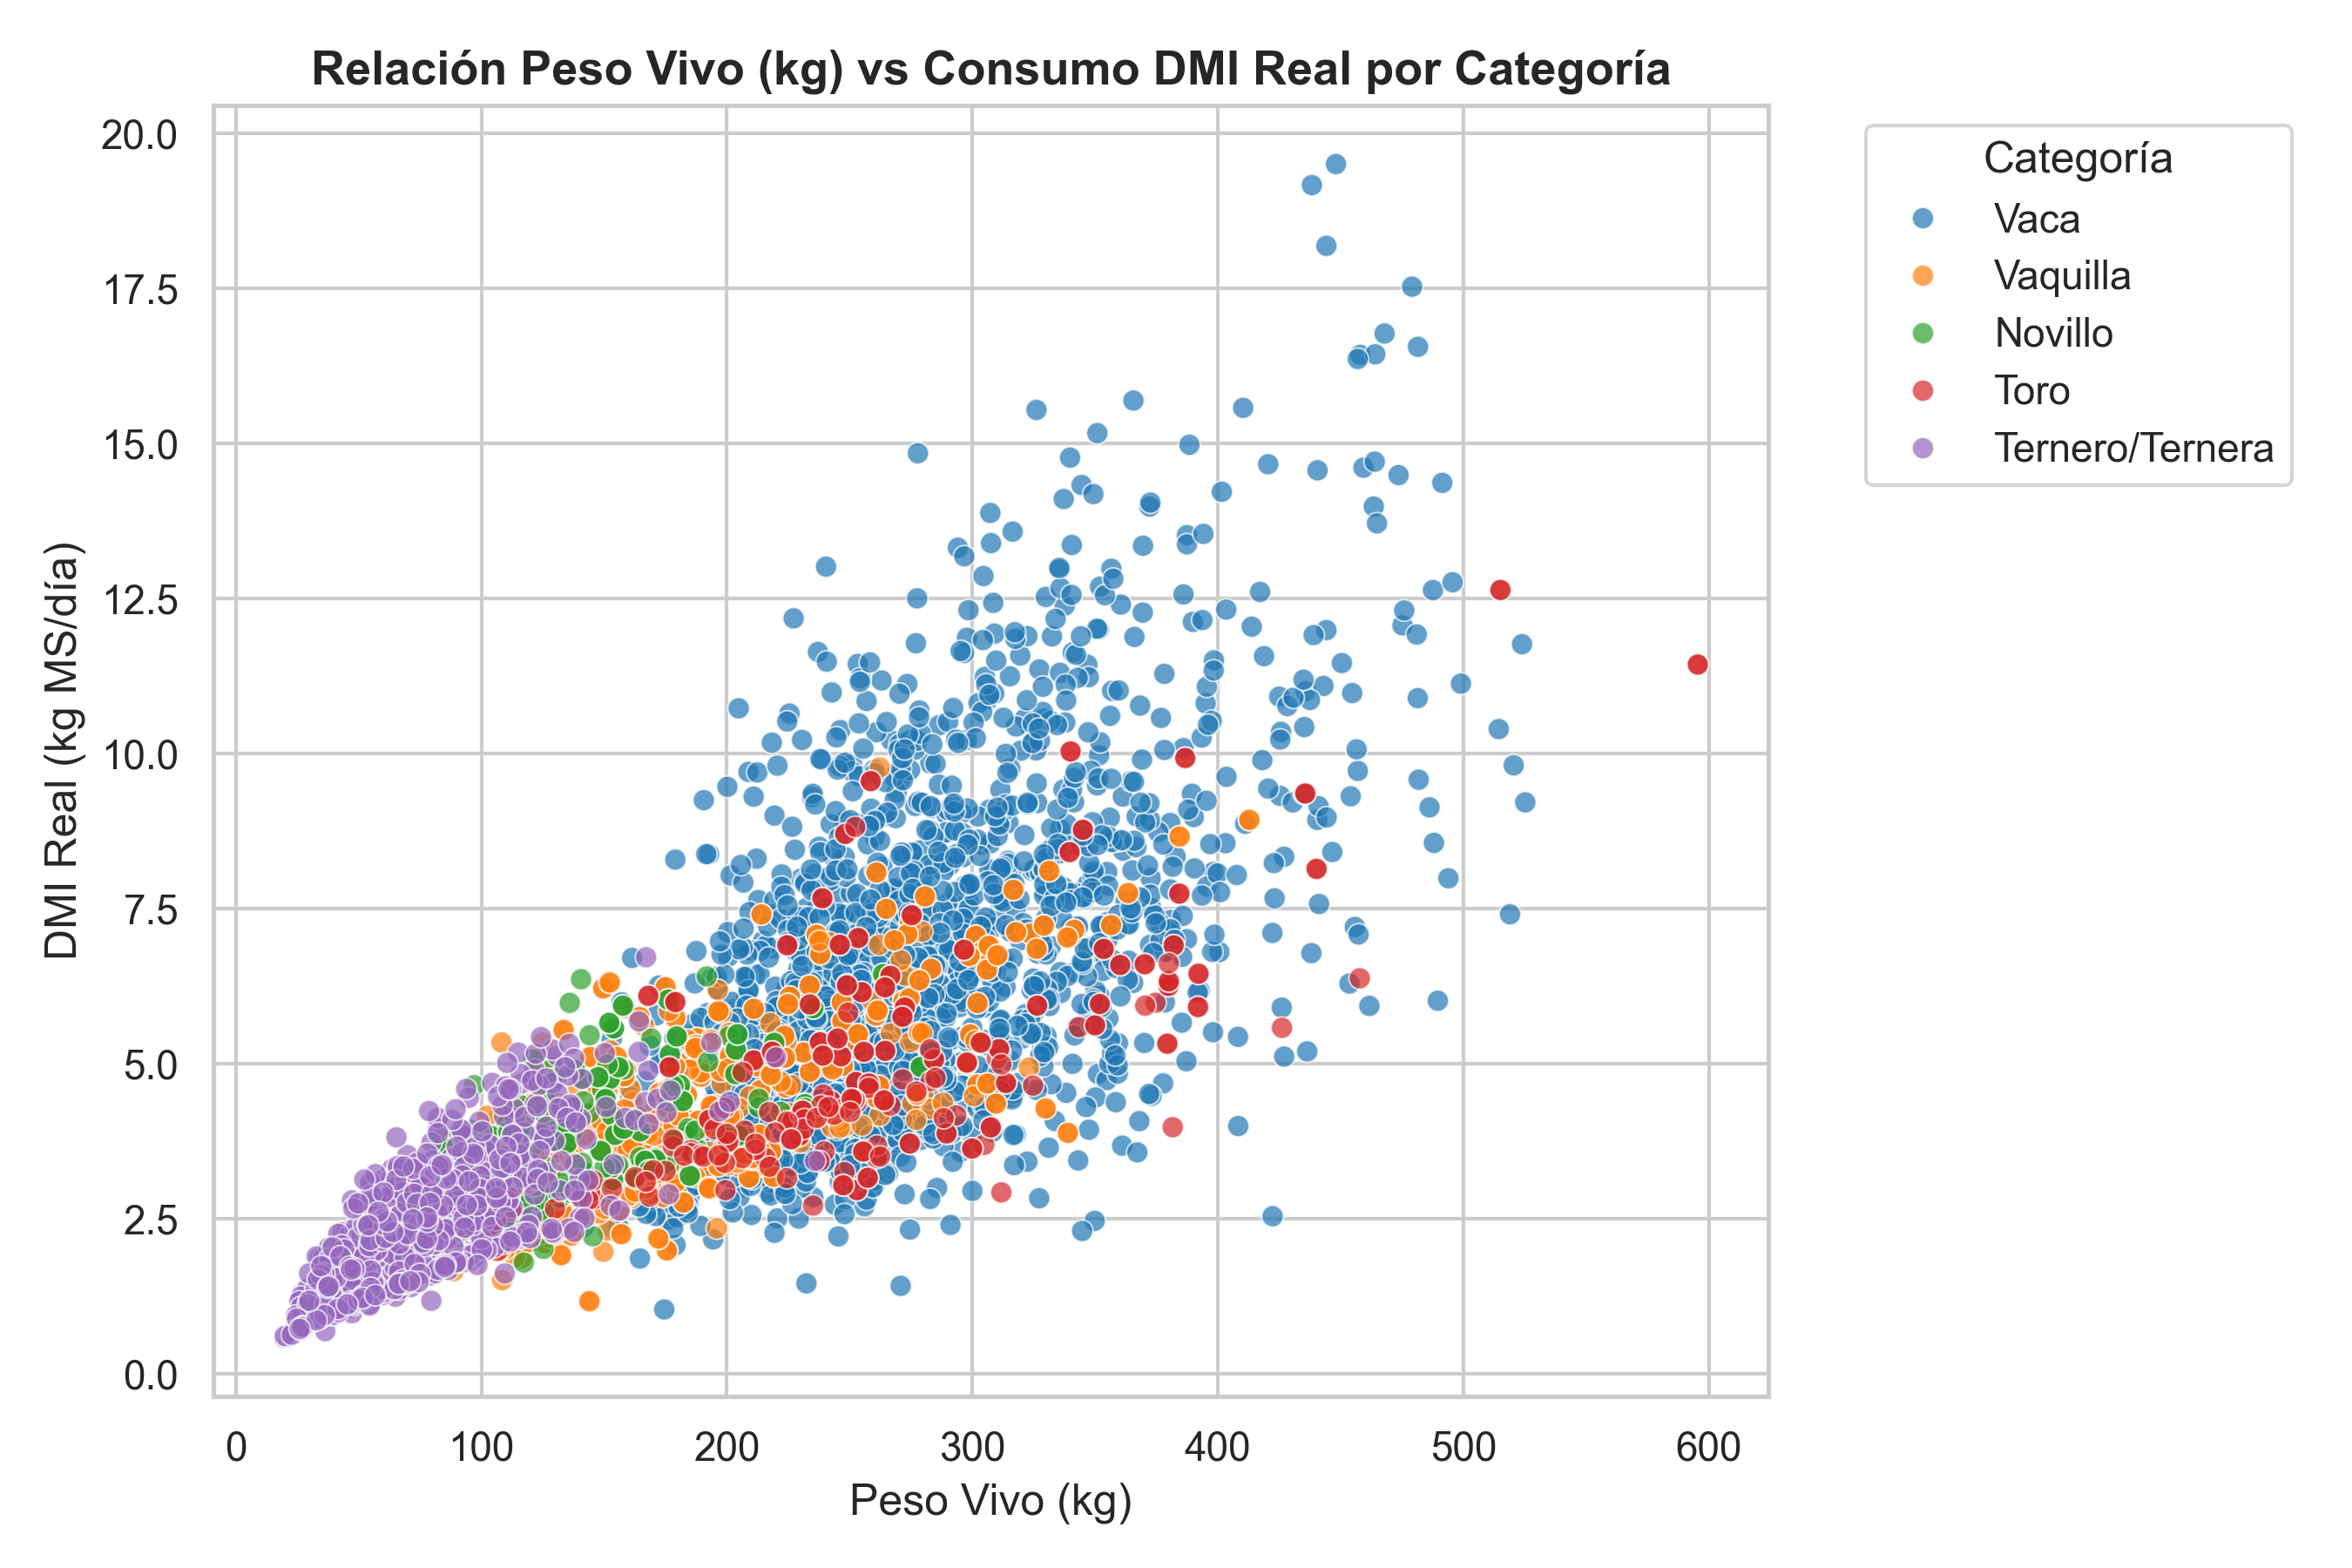
\includegraphics[width=0.86\textwidth]{figures/6_weight_vs_dmi_scatter.png}
\caption{Peso vivo y consumo real, diferenciados por categoría.}
\end{figure}

El eje horizontal es el peso y el vertical el DMI real. La nube presenta una relación positiva: en general, animales más pesados consumen más materia seca. Las categorías ocupan regiones diferentes y se superponen parcialmente. La dispersión aumenta en pesos altos, lo que indica que el peso por sí solo no explica todo el consumo. El gráfico describe asociación, no causalidad.

\subsection{Distribución de DMI por categoría}

\begin{figure}[H]
\centering
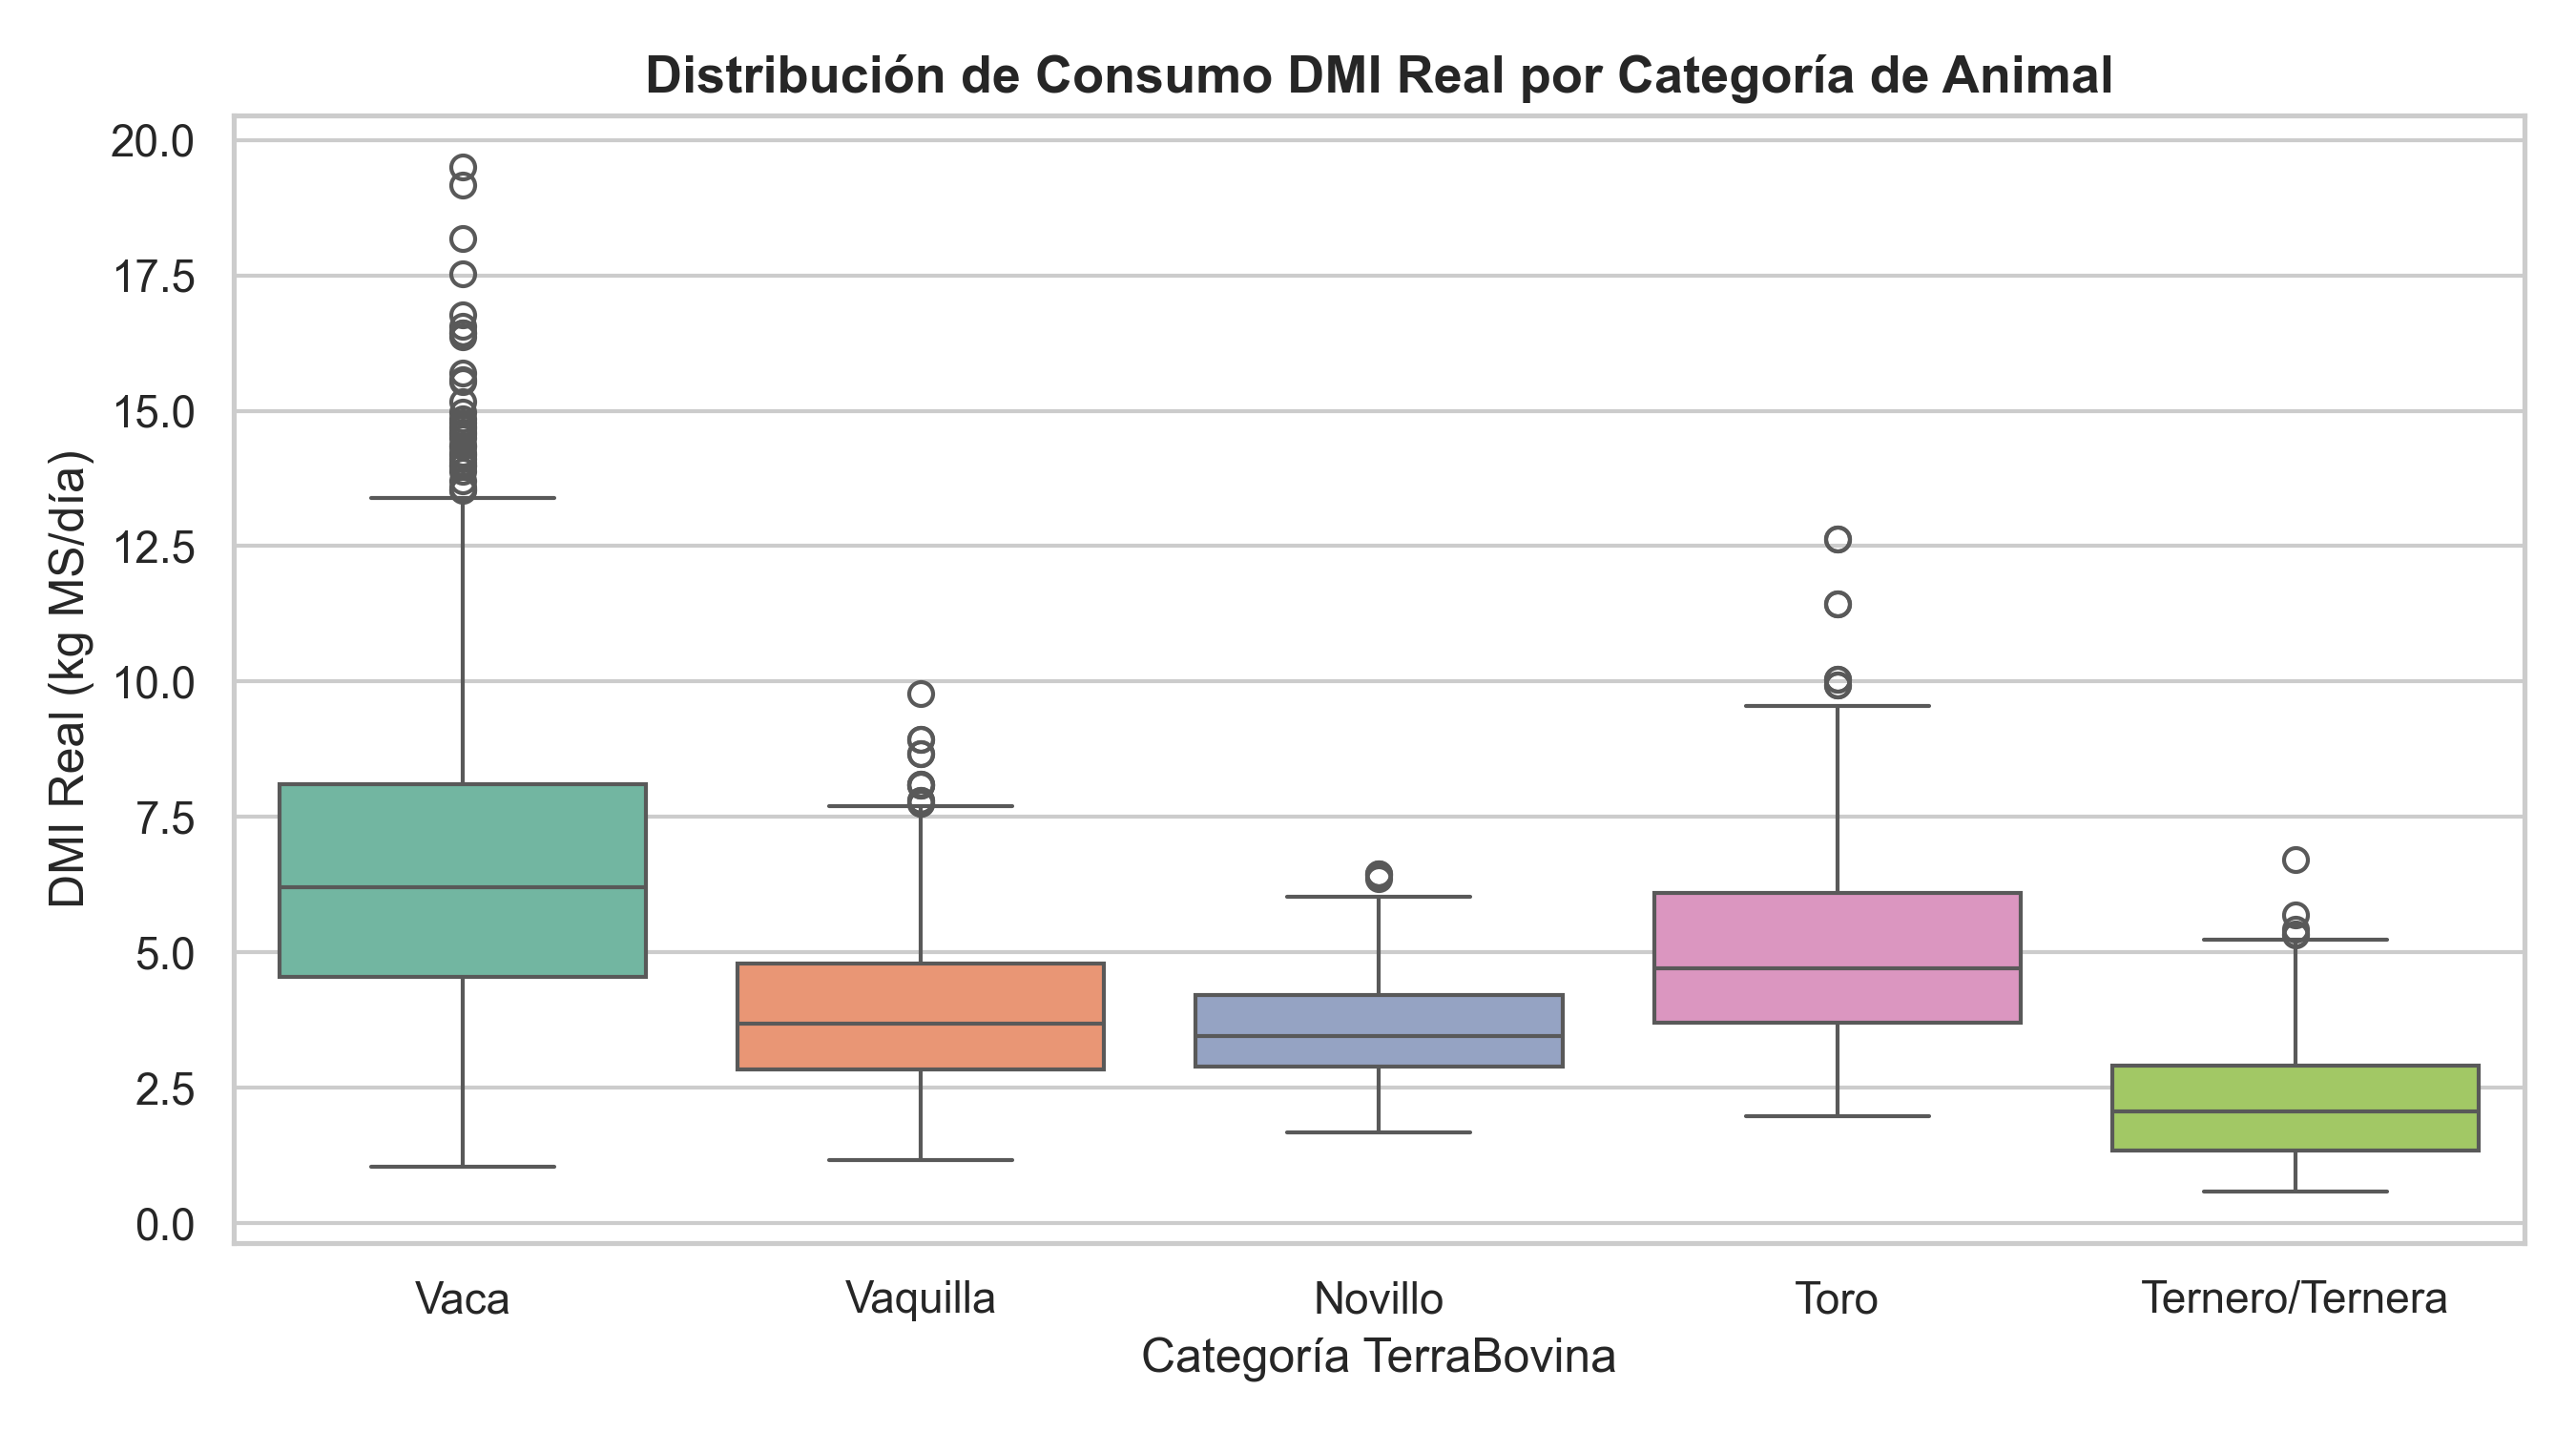
\includegraphics[width=0.86\textwidth]{figures/7_dmi_by_category_boxplot.png}
\caption{Mediana, rango intercuartílico, bigotes y valores extremos por categoría.}
\end{figure}

La línea central de cada caja es la mediana; la caja contiene la mitad central de observaciones; los puntos alejados son valores extremos según la regla del boxplot. Vaca presenta el consumo típico más alto, mayor amplitud y numerosos valores elevados. Ternero/Ternera tiene el nivel más bajo y una distribución más compacta. Esta diferencia de escala ayuda a entender por qué el MAE absoluto de vacas es mayor.

\subsection{Mapa de correlaciones}

\begin{figure}[H]
\centering
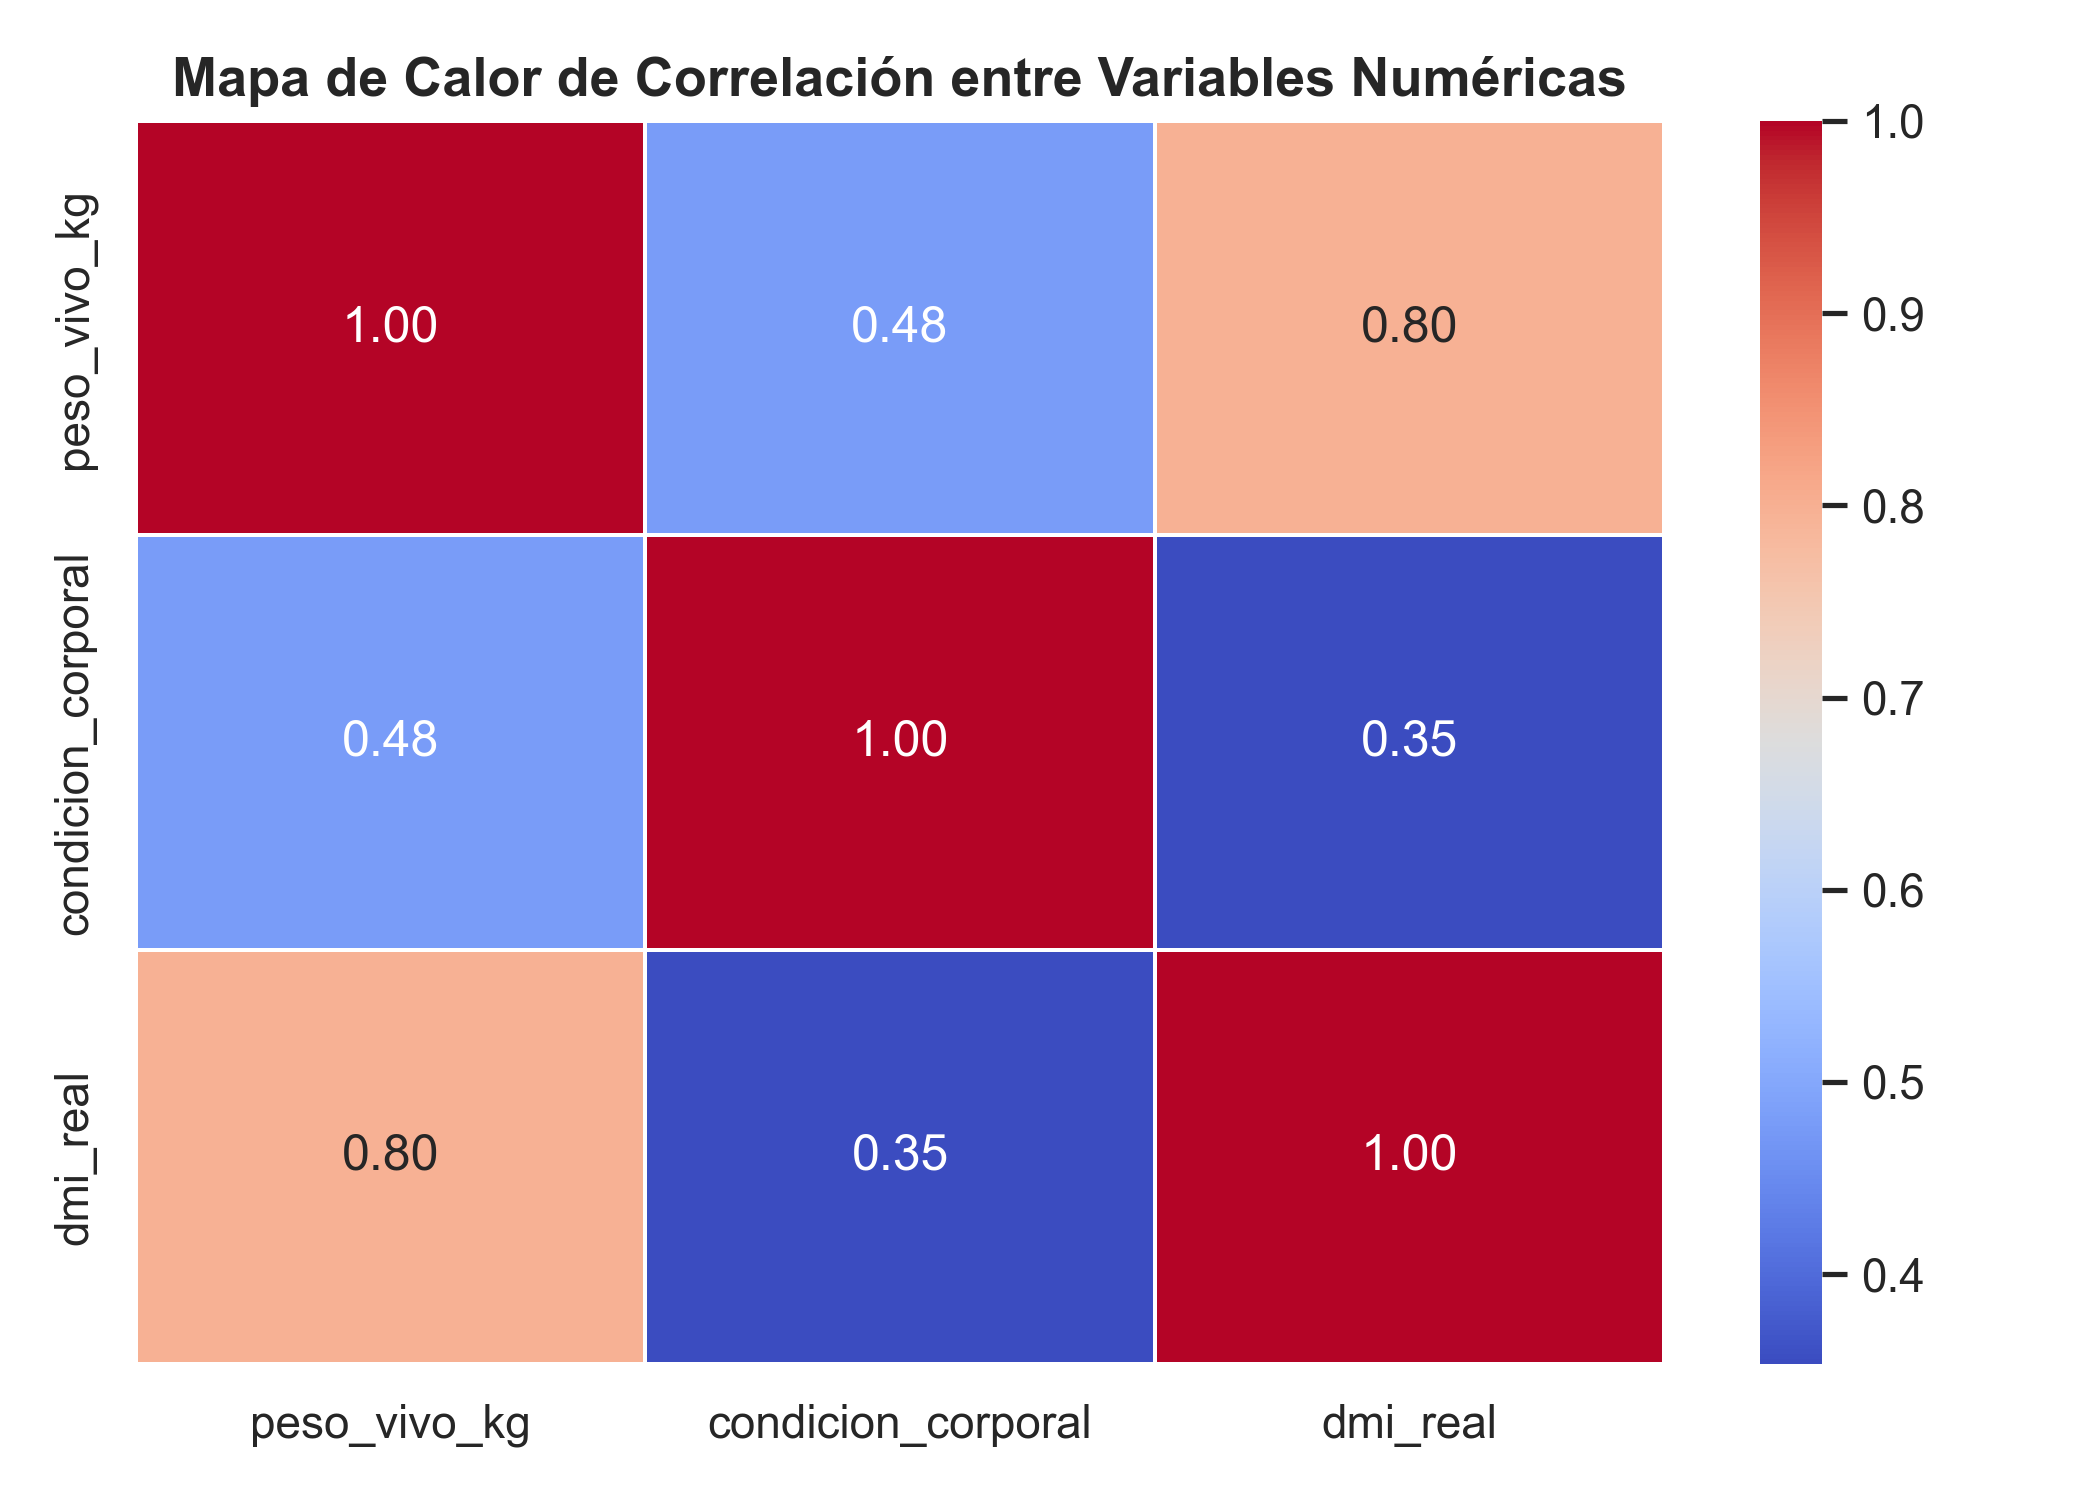
\includegraphics[width=0.72\textwidth]{figures/8_correlation_heatmap.png}
\caption{Correlación lineal entre peso, condición corporal y DMI real.}
\end{figure}

La diagonal vale 1 porque cada variable está perfectamente correlacionada consigo misma. Peso y DMI presentan correlación 0,80, fuerte y positiva. Condición corporal y DMI alcanzan 0,35, asociación positiva más débil. Peso y condición tienen 0,48. El mapa explica por qué un modelo lineal basado en peso puede ser competitivo, pero no incorpora categorías, interacciones ni causalidad. La condición corporal se observa principalmente en vacas, por lo que su correlación también está influida por ese patrón de disponibilidad.

\section{Conclusión}

El sistema aprende a estimar consumo diario de materia seca a partir de cuatro variables y se evalúa evitando compartir hogares entre entrenamiento y prueba. El baseline demuestra que predecir la media es insuficiente. Random Forest confirma que una alternativa no lineal funciona, aunque no mejora a Ridge. CatBoost obtiene un rendimiento casi idéntico al ganador y es especialmente competitivo en Ternero/Ternera.

Ridge fue elegido porque obtiene simultáneamente el menor MAE (1,1019), el menor RMSE (1,5354) y el mayor $R^2$ (0,6821), y porque ofrece simplicidad e interpretabilidad. Estos resultados son buenos frente al baseline y muestran capacidad predictiva real dentro del dataset. No son perfectos: existen errores grandes, peor desempeño absoluto en vacas y variabilidad no explicada.

Los gráficos respaldan esta lectura: hay una relación fuerte entre peso y consumo, las predicciones siguen la tendencia general, los residuos se concentran cerca de cero, pero los consumos altos resultan más difíciles. La conclusión responsable es que el modelo constituye una solución técnica prometedora y correctamente comparada, aunque necesita validación externa con datos locales antes de respaldar decisiones nutricionales reales.

\end{document}
